\item \textbf{{[}DHS/PRELIM/9597/2018/P2/Q6{]} }

Carrie Car, a car accessories shop wants to sell its products through
the internet. A software house has been engaged to supply the computerised
solution. The project manager has drawn up a list of activities and
their likely duration. 
\noindent \begin{center}
\begin{tabular}{|c|c|c|}
\hline 
Activity & Description & Weeks to complete\tabularnewline
\hline 
A & Write requirement specification & 5\tabularnewline
\hline 
B & Produce program design & 5\tabularnewline
\hline 
C & Write module code & 15\tabularnewline
\hline 
D & Module testing & 10\tabularnewline
\hline 
E & Integration testing & 5 \tabularnewline
\hline 
F & Alpha testing & 3\tabularnewline
\hline 
G & Install software and acceptance testing & 5\tabularnewline
\hline 
H & Write end user training guide & 5\tabularnewline
\hline 
J & Write technical documentation & 10\tabularnewline
\hline 
K & End user training & 4\tabularnewline
\hline 
L & Sign off final system & 1\tabularnewline
\hline 
\end{tabular}
\par\end{center}
\begin{enumerate}
\item The project manager decides to construct a Program Evaluation Review
Technique (PERT) chart from this data.
\begin{center}
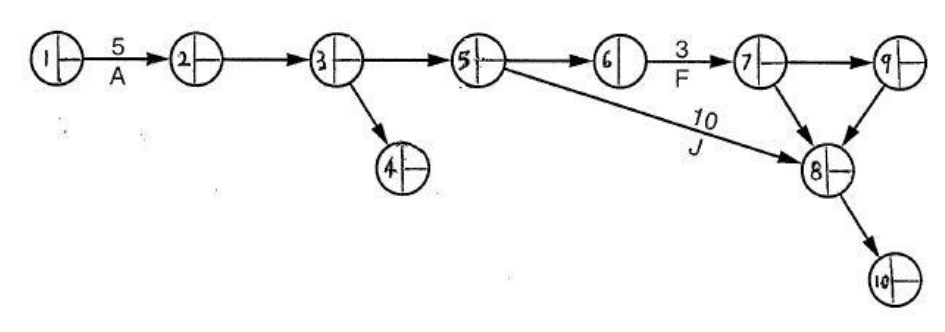
\includegraphics[width=0.5\paperwidth]{static/img/9597-HCI-2018-P2-Q6}
\par\end{center}
\begin{enumerate}
\item Complete the PERT chart. \hfill{}{[}3{]}
\item State the critical path and elapsed time for this project. \hfill{}{[}2{]}
\item State the earliest and late start for activity J. \hfill{}{[}2{]}
\end{enumerate}
\item The systems analyst from the team gathered the following requirements: 
\begin{itemize}
\item A customer can place an order either by telephone or via the internet
\item The order will be placed in a file to be dealt with by the warehouse
staff 
\item An email acknowledgement of the order will be sent to the customer 
\item After completion of the order the customer details will be stored
in a customer file 
\end{itemize}
List details of the data stores required, and draw the data flow diagram
for the solution.\hfill{} {[}6{]}
\item Various procedures are written. One of the procedures is written to
look up the customer record in the customer file. The procedure then
adds the value of the current order to the total ordered by the customer
this year. This determines whether or not a discount is payable. 

Parameters can be passed to a procedure by using pass-by-value or
pass-by-reference. Explain the two methods and highlight the difference.
Using the scenario above, give an example of each to illustrate the
difference. \hfill{}{[}6{]}
\item Besides car accessories, Carrie Car also sells car insurance. Customers
can insure their car using one of two methods: 
\begin{itemize}
\item Method A: by using the Internet or 
\item Method B: by using the telephone to talk to a sales representative. 
\end{itemize}
\begin{enumerate}
\item For method A, describe how the car registration could be validated.
\hfill{}{[}1{]}
\item For method B, describe how the car registration could be verified.
\hfill{}{[}1{]}
\item Explain the difference between data validation and data verification.
\hfill{}{[}2{]}
\end{enumerate}
\item The rules that are used when deciding whether to offer insurance to
customers and whether to offer discounts are as follows:
\begin{itemize}
\item If the customer has been refused insurance by another company and
their car is over 10 years old then insurance is refused.
\item If the customer has been refused insurance by another company and
their car is not more than 10 years old then insurance without any
discount is available. 
\item If the customer has not been refused insurance by another company
and their car is over 10 years old then insurance without any discount
is available. 
\item If the customer has not been refused insurance by another company
and their car is less than 10 years old and they have made not more
than three claims previously then insurance with a discount is available.
\begin{enumerate}
\item Create a decision table showing all the possible outcomes and results. 
\item Simplify your decision table by removing redundancies. \hfill{}{[}7{]}
\end{enumerate}
\end{itemize}